\section{Sobolev 空间}
\label{chap:sobolev-spaces}
\renewcommand{\thestatement}{1.\arabic{statement}}
\renewcommand{\thefigure}{III.\arabic{figure}}
\setcounter{figure}{0}

本章首先给出 $\mathbb{R}^d$ 中区域的基本定义与性质, 特别研究 Lipschitz 区域上的边界积分、外法向量和 Stokes 公式. 随后定义并研究这些区域上的 Sobolev 空间, 包括光滑函数稠密性、迹理论、Sobolev 嵌入以及 Poincar\'e 和 Hardy 不等式. 第 3 节研究光滑区域边界邻域的切向和法向坐标, 包括符号距离及其正则化. 最后研究带 Dirichlet 或 Neumann 边界条件的 Laplace 问题.

\subsection{区域}
\label{sec:chap3-domains}

对开集 $\Omega$, 仍以式\eqref{eq:chap2-signed-distance}中的 $\delta(x)$ 表示到 $\partial\Omega$ 的符号距离. 对 $\xi\geq0$, 记
\[
 O_\xi=\{x\in\Omega:\delta(x)<\xi\},
 \qquad\Omega_\xi=\{x\in\Omega:\delta(x)>\xi\}.
\]

\subsubsection{一般定义}
\label{subsec:chap3-domain-general-definitions}

以下 $k$ 为非负整数, $\alpha\in[0,1]$, 且 $k+\alpha\geq1$.

\begin{Definition}[$C^{k,\alpha}$ half-spaces]
\label{def:chap3-ckalpha-half-space}
对紧支集的 $C^{k,\alpha}$ 映射 $a:\mathbb{R}^{d-1}\to\mathbb{R}$, 定义
\[
 H_a=\{(\bar x,x_d)\in\mathbb{R}^d:x_d>a(\bar x)\},
\]
称为 $\mathbb{R}^d$ 中的 $C^{k,\alpha}$ 半空间. $\mathbb{R}_+^d=\mathbb{R}^{d-1}\times\mathbb{R}_+^*=H_0$ 称为平坦半空间.
\end{Definition}

\begin{Definition}
\label{def:chap3-ckalpha-domain}
若对每个 $\sigma\in\partial\Omega$, 存在开邻域 $U_\sigma$, 旋转 $R_\sigma\in O_d^+(\mathbb{R})$ 以及 $C^{k,\alpha}$ 半空间 $H_{a_\sigma}$, 使
\[
 \Omega\cap U_\sigma=(R_\sigma H_{a_\sigma})\cap U_\sigma,
 \quad
 \partial\Omega\cap U_\sigma=(R_\sigma\partial H_{a_\sigma})\cap U_\sigma,
\]
且 $\Omega^c\cap U_\sigma=(R_\sigma H_{a_\sigma}^c)\cap U_\sigma$, 则称 $\Omega$ 为 $C^{k,\alpha}$ 区域. $k=0,\alpha=1$ 时称为 Lipschitz 区域.
\end{Definition}

\begin{figure}[H]
\centering
\begin{tikzpicture}[scale=.75]
\draw[thick] (-4,-.4) .. controls (-2,1.2) and (1,-1.1) .. (4,.5);
\fill[ZhengWen,opacity=.12] (-4,-.4) .. controls (-2,1.2) and (1,-1.1) .. (4,.5) -- (4,2.6) -- (-4,2.6) -- cycle;
\draw[dashed] (-1.2,-1.5) rectangle (1.6,1.7);
\node at (-2.8,1.8) {$\Omega$}; \node at (.2,-1.8) {$U_\sigma$}; \fill (.2,.15) circle (2pt) node[below] {$\sigma$};
\end{tikzpicture}
\caption{$C^{k,\alpha}$ 区域局部为 $C^{k,\alpha}$ 半空间.}
\label{fig:chap3-local-half-space-domain}
\end{figure}

\subsubsection{Lipschitz 区域}
\label{subsec:chap3-lipschitz-domains}

\paragraph{Lipschitz 半空间}

固定磨光核 $\eta:\mathbb{R}^{d-1}\to\mathbb{R}$, 并令
\[
 M_\eta=\int_B|z|\eta(z)\,\mathrm{d}z,
 \qquad M_{\nabla\eta,k}=\int_B|z|^k|\nabla\eta(z)|\,\mathrm{d}z.
\]
取 $\gamma>0$ 使 $\gamma\operatorname{Lip}(a)M_\eta\leq1/2$, 并定义
\begin{equation}
 a_\gamma(\bar x,x_d)
 =(a*\eta_{\gamma|x_d|})(\bar x)
 =\int_Ba(\bar x-\gamma|x_d|z)\eta(z)\,\mathrm{d}z.
 \label{eq:chap3-regularized-graph}
\end{equation}

\begin{Proposition}
\label{prop:chap3-regularized-graph-properties}
$a_\gamma$ 在 $x_d\neq0$ 处光滑, $a_\gamma(\bar x,0)=a(\bar x)$, 并满足
\[
 |\partial_{x_d}a_\gamma|\leq\gamma\operatorname{Lip}(a)M_\eta,
 \quad |\partial_{x_i}a_\gamma|\leq\operatorname{Lip}(a),
 \quad |\partial_{x_i}\partial_{x_j}a_\gamma|\leq C_\gamma|x_d|^{-1}.
\]
在 $a$ 的每个可微点, $\partial_{x_i}a_\gamma(\bar x,x_d)\to\partial_{x_i}a(\bar x)$ 当 $x_d\to0$. 对固定 $\bar x$, 映射 $x_d\mapsto x_d+a_\gamma(\bar x,x_d)$ 单调递增且映满 $\mathbb{R}$. 映射
\[
 T_a(\bar x,x_d)=(\bar x,x_d+a_\gamma(\bar x,x_d))
\]
是 $\mathbb{R}^d$ 上的 Lipschitz 微分同胚, 把 $\mathbb{R}_+^d$, $\mathbb{R}_-^d$ 和 $\partial\mathbb{R}_+^d$ 分别映到 $H_a$, $H_a^c$ 和 $\partial H_a$. 其 Jacobian 行列式及逆映射的 Jacobian 行列式分别位于 $[1/2,3/2]$ 和 $[2/3,2]$.
\end{Proposition}

\begin{Proof}
正则性和极限由 Proposition~\ref{prop:chap2-mollification-lipschitz} 得到. 利用 $a$ 的 Lipschitz 性可得一阶导数估计; 对卷积表达式求导并使用 $\int\partial_i\eta=0$ 与 $\int z\cdot\nabla\eta=-(d-1)$, 得二阶导数估计. 又
\[
 (y_1+a_\gamma(\bar x,y_1))-(y_2+a_\gamma(\bar x,y_2))
 \geq(1-\gamma\operatorname{Lip}(a)M_\eta)|y_1-y_2|,
\]
从而得到单调性、满射性和 $T_a$ 的可逆性. 最后 $J_{T_a}=1+\partial_{x_d}a_\gamma$ 给出 Jacobian 估计.
\end{Proof}

\paragraph{锥性质及其推论}

\begin{Theorem}
\label{thm:chap3-lipschitz-cone-property}
边界紧的 Lipschitz 区域 $\Omega\subset\mathbb{R}^d$ 满足锥性质: 存在 $\partial\Omega$ 的有限开覆盖 $(U_i)_{1\leq i\leq N}$、$\theta\in(0,\pi/2)$ 和 $\delta_0>0$, 使 $O_{\delta_0}\subset\bigcup_iU_i$, 且对每个 $i$ 存在单位向量 $\widetilde\nu_i$, 若
\[
 C_i=\{z\in\mathbb{R}^d:\sin\theta|z|\leq z\cdot\widetilde\nu_i\leq\delta_0\},
\]
则
\begin{equation}
 x+C_i\subset\Omega\quad(x\in\Omega\cap U_i),
 \qquad x-C_i\subset\Omega^c\quad(x\in\Omega^c\cap U_i),
 \label{eq:chap3-cone-property}
\end{equation}
并且
\begin{equation}
 x-t\widetilde\nu_i\in U_i,
 \quad x\in\Omega\cap U_i,\quad0\leq t\leq\delta_0/2.
 \label{eq:chap3-cone-cover-shift}
\end{equation}
\end{Theorem}

\begin{figure}[H]
\centering
\begin{tikzpicture}[scale=.62]
\draw[thick] (-4,0) .. controls (-2,1) and (1,-1) .. (4,.2);
\fill[ZhengWen,opacity=.10] (-4,0) .. controls (-2,1) and (1,-1) .. (4,.2) -- (4,2.5) -- (-4,2.5) -- cycle;
\draw[->,thick] (0,0) -- (0,2) node[above] {$\widetilde\nu$};
\draw[dashed] (0,0) -- (-1.3,1.8); \draw[dashed] (0,0) -- (1.3,1.8);
\node at (2.7,1.6) {$H_a$};
\end{tikzpicture}
\caption{半空间 $H_a$ 及其内锥.}
\label{fig:chap3-half-space-cone}
\end{figure}

\begin{Proof}
由边界紧性只需在一个 Lipschitz 半空间 $H_a$ 上证明. 取 $\widetilde\nu=e_d$, $\theta=\arctan(\operatorname{Lip}(a))$, 并取
\begin{equation}
 U=\bigcup_{|\bar x|<\alpha}\{\bar x\}\times(a(\bar x)-\alpha,a(\bar x)+\alpha).
 \label{eq:chap3-local-cylinder}
\end{equation}
若 $y-x$ 位于对应的无限锥中, 则 Lipschitz 估计给出 $y_d>a(\bar y)$, 故 $x+C\subset H_a$; 补集情形相同. 取充分小的 $\delta_0<2\alpha$ 即得式\eqref{eq:chap3-cone-cover-shift}.
\end{Proof}

令 $U_0=\Omega_{\delta_0/2}$ 和 $\nu_0=0$.

\begin{Proposition}
\label{prop:chap3-shifted-balls-cone}
在 Theorem~\ref{thm:chap3-lipschitz-cone-property} 的记号下, 存在 $M>0$ 和 $\varepsilon_0>0$, 使对 $\nu_i=M\widetilde\nu_i$ 和 $0<\varepsilon<\varepsilon_0$:
\begin{equation}
 B(y+\varepsilon\nu_i,\varepsilon)
 \subset B(y+\varepsilon\nu_i,2\varepsilon)\subset\Omega,
 \quad y\in U_i\cap\Omega,
 \label{eq:chap3-inward-shifted-ball}
\end{equation}
且对 $i\geq1$ 及 $y\in U_i$ 满足 $d(y,\partial\Omega)\leq\varepsilon/M$,
\begin{equation}
 B(y-\varepsilon\nu_i,\varepsilon)\subset\Omega^c.
 \label{eq:chap3-outward-shifted-ball}
\end{equation}
\end{Proposition}

\begin{figure}[H]
\centering
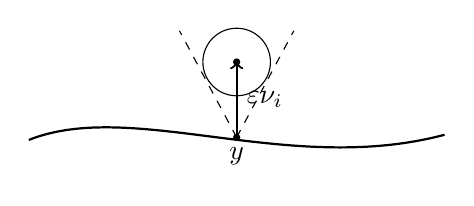
\begin{tikzpicture}[scale=.66]
\draw[thick] (-4,0) .. controls (-2,.8) and (1,-.7) .. (4,.1);
\fill (0,.05) circle (2pt) node[below] {$y$};
\draw[->,thick] (0,.05) -- (0,1.5) node[midway,right] {$\varepsilon\nu_i$};
\draw (0,1.5) circle (.65); \fill (0,1.5) circle (2pt);
\draw[dashed] (0,.05) -- (-1.1,2.1); \draw[dashed] (0,.05) -- (1.1,2.1);
\end{tikzpicture}
\caption{球 $B(y+\varepsilon\nu_i,2\varepsilon)$ 包含于锥 $C_i$.}
\label{fig:chap3-shifted-ball-in-cone}
\end{figure}

\begin{Proof}
取 $M>2$ 使 $\sin^2\theta=(M^2-4)/M^2$, 并令 $\varepsilon_0=\delta_0/(M+2)$. 对 $i\geq1$, 直接验证 $B(\varepsilon M\widetilde\nu_i,2\varepsilon)\subset C_i$, 再用式\eqref{eq:chap3-cone-property}得到第一式. 对第二式, 沿 $-\nu_i$ 方向把 $y$ 移到 $U_i\cap\Omega^c$, 再应用同一锥论证. $i=0$ 的情形由 $U_0$ 到边界的距离得到.
\end{Proof}

\begin{Definition}
\label{def:chap3-star-shaped}
若存在 $x_0\in A$ 使对每个 $x\in A$, 线段 $[x_0,x]\subset A$, 则称 $A$ 关于 $x_0$ 星形.
\end{Definition}

\begin{Lemma}
\label{lem:chap3-lipschitz-locally-star-shaped}
有界 Lipschitz 区域 $\Omega$ 可由有限个星形开集覆盖. 无界 Lipschitz 区域可由局部有限的星形开集族覆盖.
\end{Lemma}

\begin{Proof}
内部点附近可取包含于 $\Omega$ 的球. 对 $a\in\partial\Omega\cap U_i$, 取
\[
 O=\bigcup_{x\in\partial\Omega\cap U_i,\ |x-a|<\varepsilon}
 (x+\mathring C_i\cup\{0\}).
\]
当 $\varepsilon$ 充分小时, $O$ 关于 $a+(\delta_0/2)\widetilde\nu_i$ 星形. 紧性给出有限覆盖, 无界情形给出局部有限覆盖.
\end{Proof}

\paragraph{Lipschitz 区域边界上的积分}

对 Lipschitz 半空间 $H_a$ 和紧支集连续函数 $\varphi$, 定义
\begin{equation}
 \int_{\partial H_a}\varphi\,\mathrm{d}\sigma
 =\int_{\mathbb{R}^{d-1}}\varphi(\bar x,a(\bar x))J_a(\bar x)\,\mathrm{d}\bar x,
 \quad
 J_a=\sqrt{1+\sum_{i=1}^{d-1}(\partial_{x_i}a)^2}.
 \label{eq:chap3-boundary-integral-half-space}
\end{equation}
由 Theorem~\ref{thm:chap2-rademacher}, $J_a$ 几乎处处有定义. 外单位法向量为
\begin{equation}
 \nu_{H_a}(\bar x,a(\bar x))
 =\frac1{J_a(\bar x)}
 (\partial_{x_1}a,\ldots,\partial_{x_{d-1}}a,-1)^T.
 \label{eq:chap3-outward-normal-half-space}
\end{equation}
对一般边界紧的 Lipschitz 区域, 通过有限图覆盖和单位分解定义 $\partial\Omega$ 上的 Radon 测度 $\mathrm{d}\sigma$ 及外单位法向量 $\nu\in(L^\infty(\partial\Omega))^d$; 该定义与覆盖、图和单位分解的选择无关.

\paragraph{Stokes 公式}

\begin{Theorem}[Stokes formula. Divergence theorem]
\label{thm:chap3-stokes-divergence}
设 $\Omega\subset\mathbb{R}^d$ 为边界紧的 Lipschitz 区域. 对任意 $\Phi\in(C_c^1(\mathbb{R}^d))^d$,
\begin{equation}
 \int_\Omega\operatorname{div}\Phi\,\mathrm{d}x
 =\int_{\partial\Omega}\Phi\cdot\nu\,\mathrm{d}\sigma.
 \label{eq:chap3-stokes-divergence}
\end{equation}
因此对 $\psi\in C_c^1(\mathbb{R}^d)$,
\begin{equation}
 \int_\Omega\psi\operatorname{div}\Phi\,\mathrm{d}x
 +\int_\Omega\Phi\cdot\nabla\psi\,\mathrm{d}x
 =\int_{\partial\Omega}\psi\Phi\cdot\nu\,\mathrm{d}\sigma.
 \label{eq:chap3-stokes-product}
\end{equation}
\end{Theorem}

\begin{Proof}
线性和单位分解把一般情形约化到 Lipschitz 半空间. 对光滑图 $a$, Fubini 定理和 $\bar x$ 方向分部积分给出
\[
 \int_{H_a}\operatorname{div}\Phi\,\mathrm{d}x
 =\int_{\mathbb{R}^{d-1}}
 \Phi(\bar x,a(\bar x))\cdot
 (\nabla a(\bar x),-1)^T\,\mathrm{d}\bar x,
\]
再用式\eqref{eq:chap3-boundary-integral-half-space}和\eqref{eq:chap3-outward-normal-half-space}得到结论.

\begin{figure}[H]
\centering
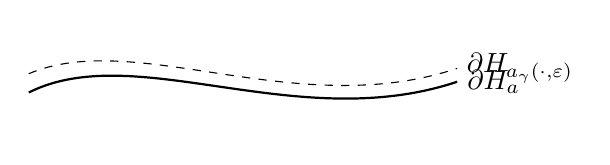
\begin{tikzpicture}[scale=.68]
\draw[thick] (-4,0) .. controls (-2,1) and (1,-.8) .. (4,.2) node[right] {$\partial H_a$};
\draw[dashed] (-4,.35) .. controls (-2,1.2) and (1,-.55) .. (4,.45) node[right] {$\partial H_{a_\gamma(\cdot,\varepsilon)}$};
\end{tikzpicture}
\caption{Lipschitz 半空间 $H_a$ 及其光滑逼近.}
\label{fig:chap3-smooth-half-space-approximation}
\end{figure}

对 Lipschitz 图, 使用式\eqref{eq:chap3-regularized-graph}构造光滑半空间 $H_{a_\gamma(\cdot,\varepsilon)}$. 当 $\varepsilon\to0$, 特征函数、图函数和几乎处处的切向导数收敛, 并具有统一有界控制. Lebesgue 控制收敛定理允许在体积分和边界积分中传递到极限, 得式\eqref{eq:chap3-stokes-divergence}. 对向量场 $\psi\Phi$ 应用该式即得式\eqref{eq:chap3-stokes-product}.
\end{Proof}
